\documentclass[12pt]{book}
\usepackage[hmargin=0.6in,vmargin=1in]{geometry}
\usepackage{amsmath}
\usepackage{amsthm}
\usepackage[rightcaption]{sidecap}
\usepackage{graphicx}
\usepackage{placeins}
\usepackage{enumerate}
\usepackage{amssymb}
\usepackage{wrapfig}
\usepackage[dvipsnames]{xcolor}
\usepackage{tikz,lipsum,lmodern}
\usepackage[most]{tcolorbox}

\title{Using fancyhdr for Custom Page Header and Footers in a Two-sided Document}

\usepackage{etoolbox}
\makeatletter
% no new page for \chapter
\patchcmd{\chapter}{\if@openright\cleardoublepage\else\clearpage\fi}{}{}{}
% don't change the pagestyle
\patchcmd{\chapter}{\thispagestyle{plain}}{}{}{%
    % example for a warning, 'Package' in text necessary to make TexStudio show it.
    \GenericWarning{(preamble)\@spaces\@spaces\@spaces\@spaces}{Package preamble Warning: patching \string\chapter\space did not work.}}

% allow floats on top of the page with a new chapter
\patchcmd{\chapter}{\global\@topnum\z@}{}{}{}
% if not commented out, first paragraph will be indented
\patchcmd{\chapter}{\@afterindentfalse}{}{}{}
%\makeatother

\usepackage{titlesec}
\titleformat{\chapter}{\normalfont\bfseries\Large}{\thechapter.\quad}{0pt}{}
\titlespacing{\chapter}{0pt}{-5pt}{4pt}% left space, top space, bottom space



\usepackage{fancyhdr}
% Clear off all default fancyhdr headers and footers
\fancyhf{}
\pagestyle{fancy}

\addtolength{\headheight}{\baselineskip}

\fancyhead[L]{\leftmark}
\renewcommand{\chaptermark}[1]{\markboth{\MakeUppercase{#1}}{}}
%\fancyhead[L]{\textbf{\sectiontitle}}
\fancyhead[R]{\sffamily\itshape Lecture Notes on Biophysics}
% Custom text at the left edge of odd pages, and right edge of odd pages.
%\fancyhead[LO,RE]{\sffamily\itshape Fun with fancyhdr}

% Repeat for \fancyfoot if needed, e.g.
% Some decorative symbol at the centre of both odd and even pages
\fancyfoot[L]{\sffamily\itshape Linn Abraham , MGM College of Nursing}
\fancyfoot[C]{\thepage}

\fancyfoot[R]{ June 2020}
% Set this length to 0pt if you don't want any lines!
\renewcommand{\headrulewidth}{2pt}
\pagenumbering{roman}
% Apply the fancy header style


\usepackage{lipsum}
\begin{document}

\title{Light}
\setcounter{page}{1}
\maketitle
\chapter{Introduction}
\begin{figure}[htpb]
    \centering
    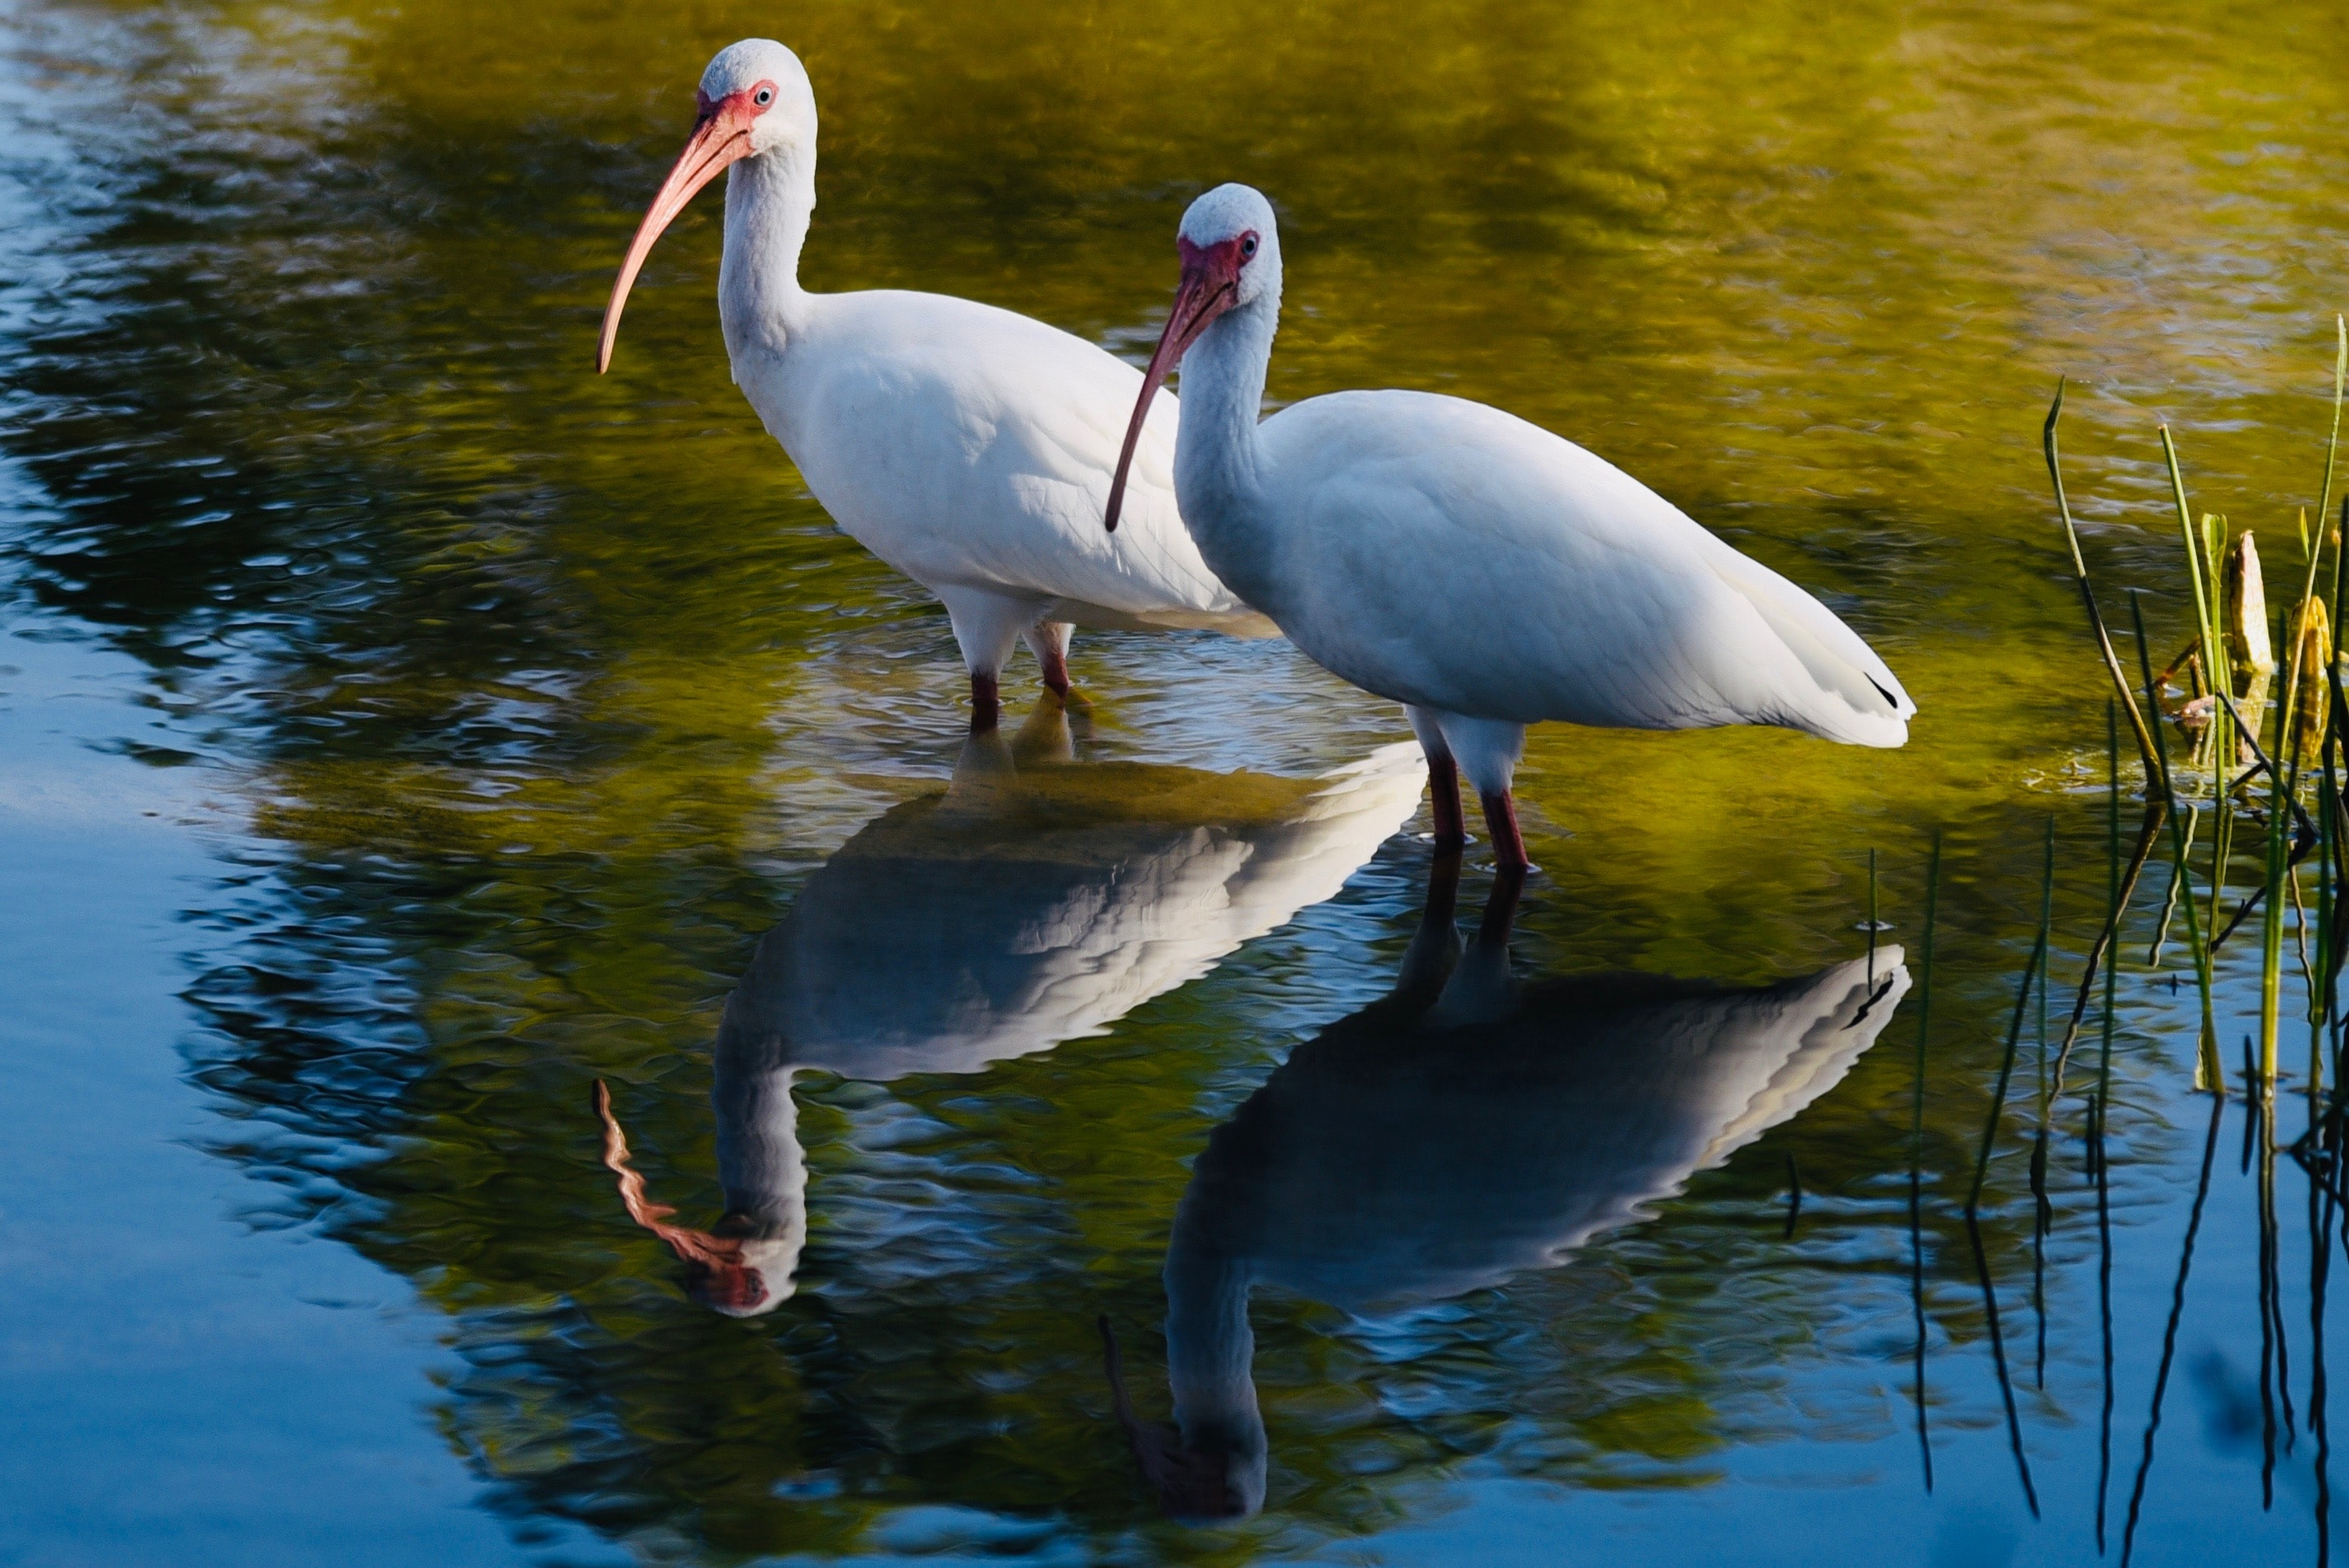
\includegraphics[width=0.8\linewidth]{../pond_reflection.jpg}
    \caption{Reflection, Refraction and Transmission of Light}%
    \label{fig:}
\end{figure}


When light falls on the interface separating two media, one or all
of the three following processes can occur :
\begin{itemize}
    \item The incident light or a part of it is turned back; that is reflected
into the first medium.
\item The incident light is partly or completely absorbed by the second
medium.
\item A fraction of the incident light is transmitted, i.e. refracted into
the second medium as in case of air water interface.
\end{itemize}

\section{Reflection}
\begin{itemize}
    \item Ability to see objects and their colours arises from reflection.
\item Mirrors make use of reflection to form images.
\item Laser pointers can be used to demonstate reflection.
\end{itemize}
\subsection*{Laws of Reflection}
When a ray of light is incident at a plane interface the angle of
incidence is equal to angle of reflection. This is known as law of
reflection.

\begin{figure}[h]
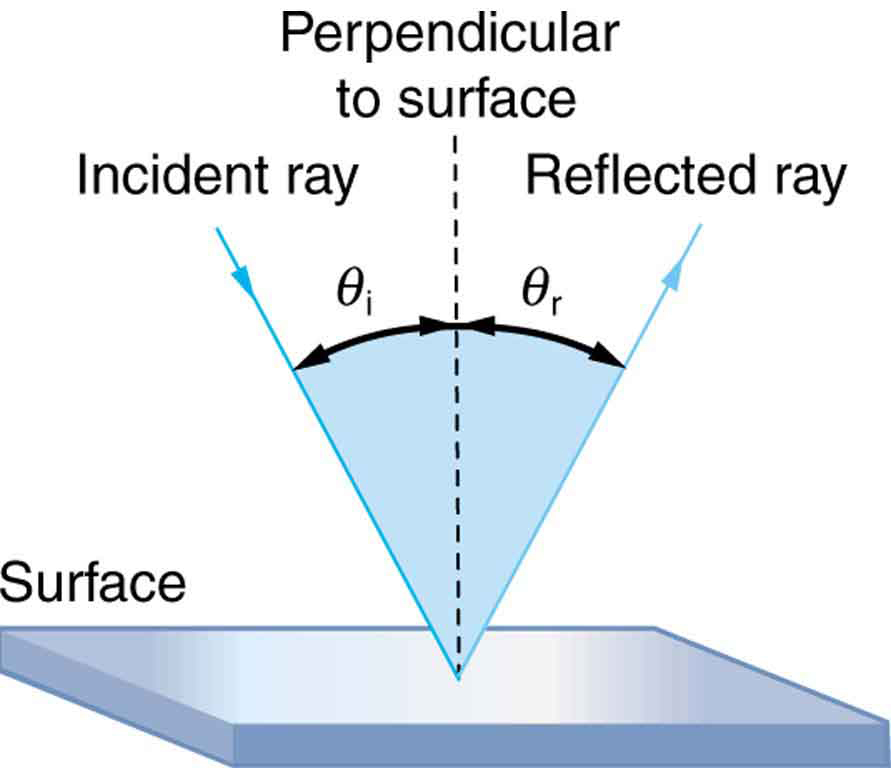
\includegraphics[scale=.70]{../lor1.jpeg}
\centering
\caption{Laws of reflection}
\end{figure}
\subsection*{Specular and Diffuse Reflection}
Reflection is of two types, specular reflection and diffuse reflection.

Specular reflection is produced from surfaces that are smoooth.
The reflection that is produced in mirrors and other smooth surfaces is specular reflection.
\begin{figure}[htpb]
    \centering
    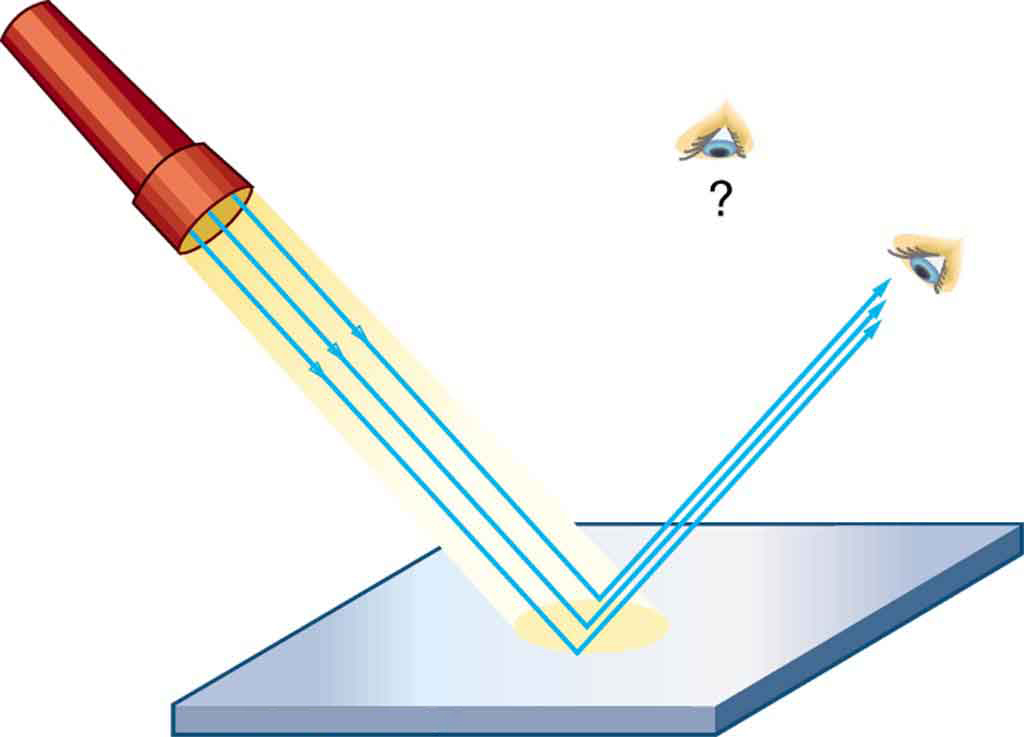
\includegraphics[width=0.5\linewidth]{../specular.jpeg}
    \caption{ A mirror illuminated by many parallel rays reflects them in only one direction, since its surface is very smooth. Only the observer at a particular angle will see the reflected light.}%
    \label{fig:}
\end{figure}
Diffuse reflection is caused from rough or uneven surfaces.
\begin{figure}[htpb]
    \centering
    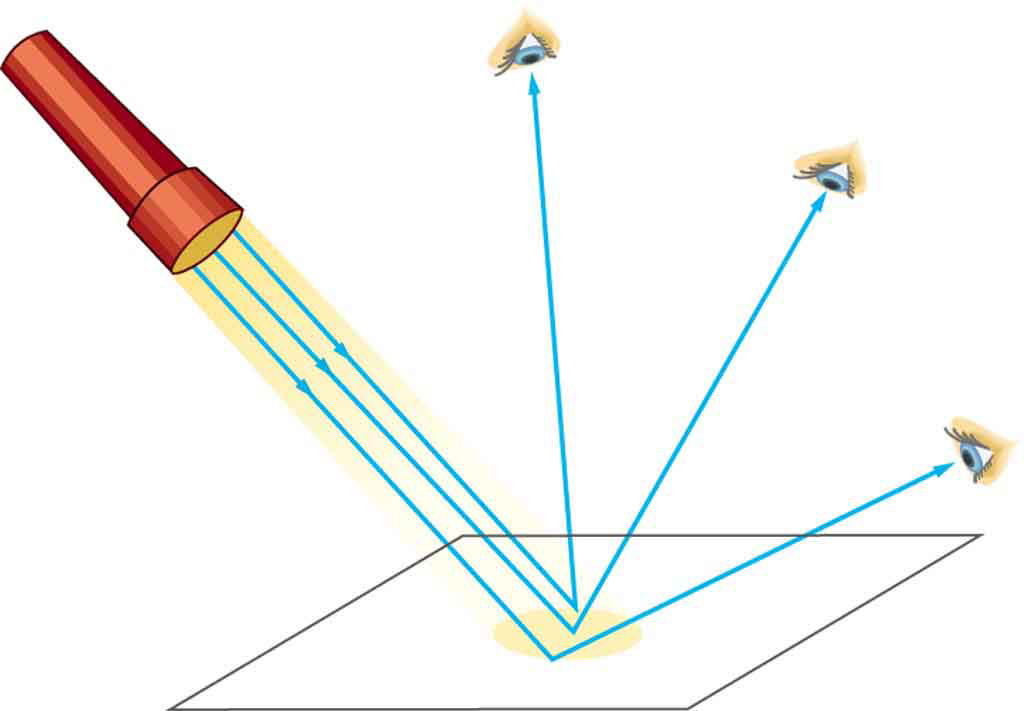
\includegraphics[width=0.5\linewidth]{../diffuse.jpeg}
    \caption{When a sheet of paper is illuminated with many parallel incident rays, it can be seen at many different angles, because its surface is rough and diffuses the light.}%
    \label{fig:}
\end{figure}
\begin{figure}[htpb]
    \centering
    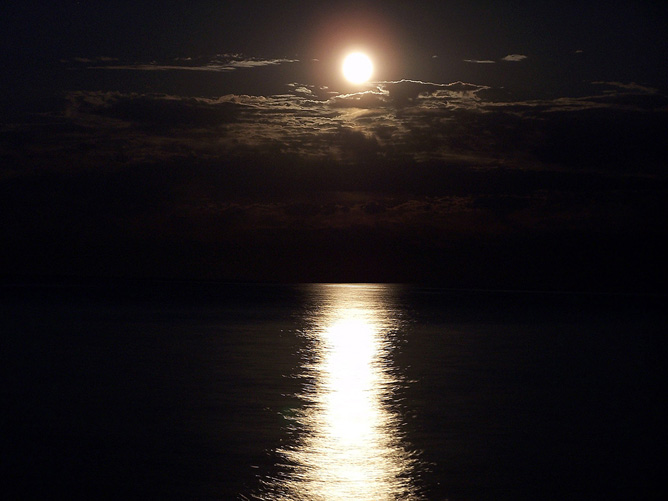
\includegraphics[width=0.8\linewidth]{../moonlight.jpeg}
    \caption{ Moonlight is spread out when it is reflected by the lake, since the surface is shiny but uneven.}%
    \label{fig:}
\end{figure}
\section{Refraction}
As you might already know light is the fastest thing in the universe. It has a speed of 3 lakh km per second. (3 x $10^{8}$ m/s). But this is its speed in vaccum.
Light has a different speed in a  different medium. When the speed of light is higher in a medium, it is called a denser medium (optically denser). If its higher in a medium it is called a rarer medium.
\subsection*{Laws of Refraction}

When rays of light travel from a rarer medium to a denser medium,
it bends toward the normal to the interface separating two media.

For a given media (for example, air or glass) the ratio of sine of angle of incidence to sine of angle of refraction is constant
for all angles of incidence. This constant is known as the refractive index
\begin{figure}[htpb]
    \centering
    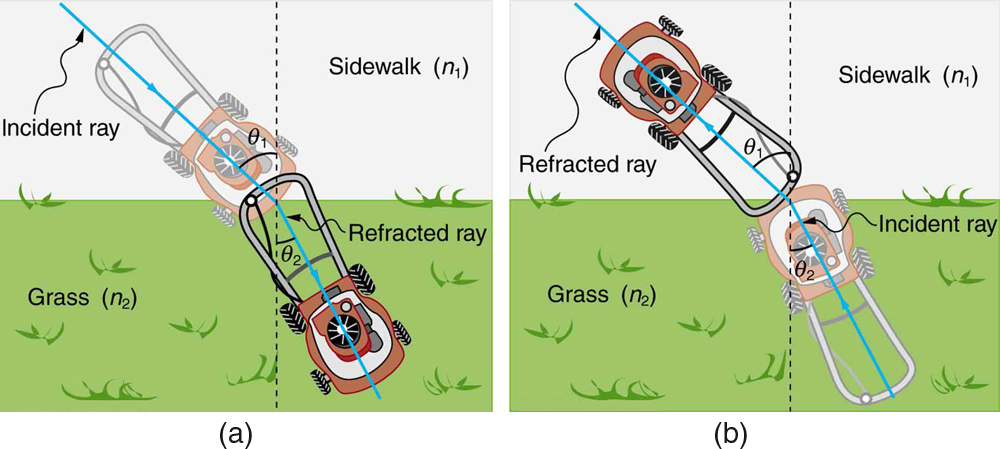
\includegraphics[width=0.8\linewidth]{../bending_light.jpeg}
    \caption{The change in direction of a light ray depends on how the speed of light changes when it crosses from one medium to another. The speed of light is greater in medium 1 than in medium 2 in the situations shown here. (a) A ray of light moves closer to the perpendicular when it slows down. This is analogous to what happens when a lawn mower goes from a footpath to grass. (b) A ray of light moves away from the perpendicular when it speeds up. This is analogous to what happens when a lawn mower goes from grass to footpath. The paths are exactly reversible.}%
    \label{fig:}
\end{figure}
\section{Lenses and Images}
\subsection{Need for lenses}
A rectangular glass slab produces  parallel emerging rays. As a result it cannot change the size of the image formed. There is no magnification. However by changing the shape of one or both sides of the slab to a different shape (concave or convex) one is able to achieve this.

A concave or convex lens is able to bend the light coming out from the glass and hence produce real or virtual images.
%\subsection{Features of Lenses}
\section{Human Eye}
\subsection{Structure of Eye}
\subsection{Action of Eye}
Light enters the eye through the hard and transparent cornea into a
fluid called aqueous humor. It then passes through the eye lens and
vitreous humor via iris. The combination of cornea, aqueous humor,
lens and vitreous humor focuses the incoming light on the retina,
in the normal eye, the principal focal point coincides with the retina
so that all objects are focused on it. The real inverted image formed
on the retina is transmitted to the brain. Most of the refraction, which
causes image formation in the retina, actually takes place at the cornea
and vitreous humor. But the focal length of the lens is adjustable and
\subsubsection{Power of Accomodation}
\subsubsection{Least distance of distant vision}
\subsection{Defects of Visions and Its Correction}
\subsubsection{Hypermetropia}
The near point is greater than 25cm. This is because the image of the objects placed at the near point are formed behind the retina.
\subsubsection{Myopia}
Cannot see distant objects clearly. The image is formed in front of the retina.
\subsubsection{Presbyopia}
This is long sightedness caused due to old age.
\subsubsection{Astigmatism}
\end{document}
